\documentclass[border=3pt,tikz]{standalone}
\usepackage[utf8]{vietnam}
\usetikzlibrary{calc,angles,intersections,shapes.geometric,arrows,decorations.markings,arrows.meta,patterns.meta,patterns}
\usepackage{tikz-3dplot,pgfplots}
\pgfplotsset{compat=1.15}
\usepgfplotslibrary{polar}
\usepackage{amsmath}
\begin{document}
	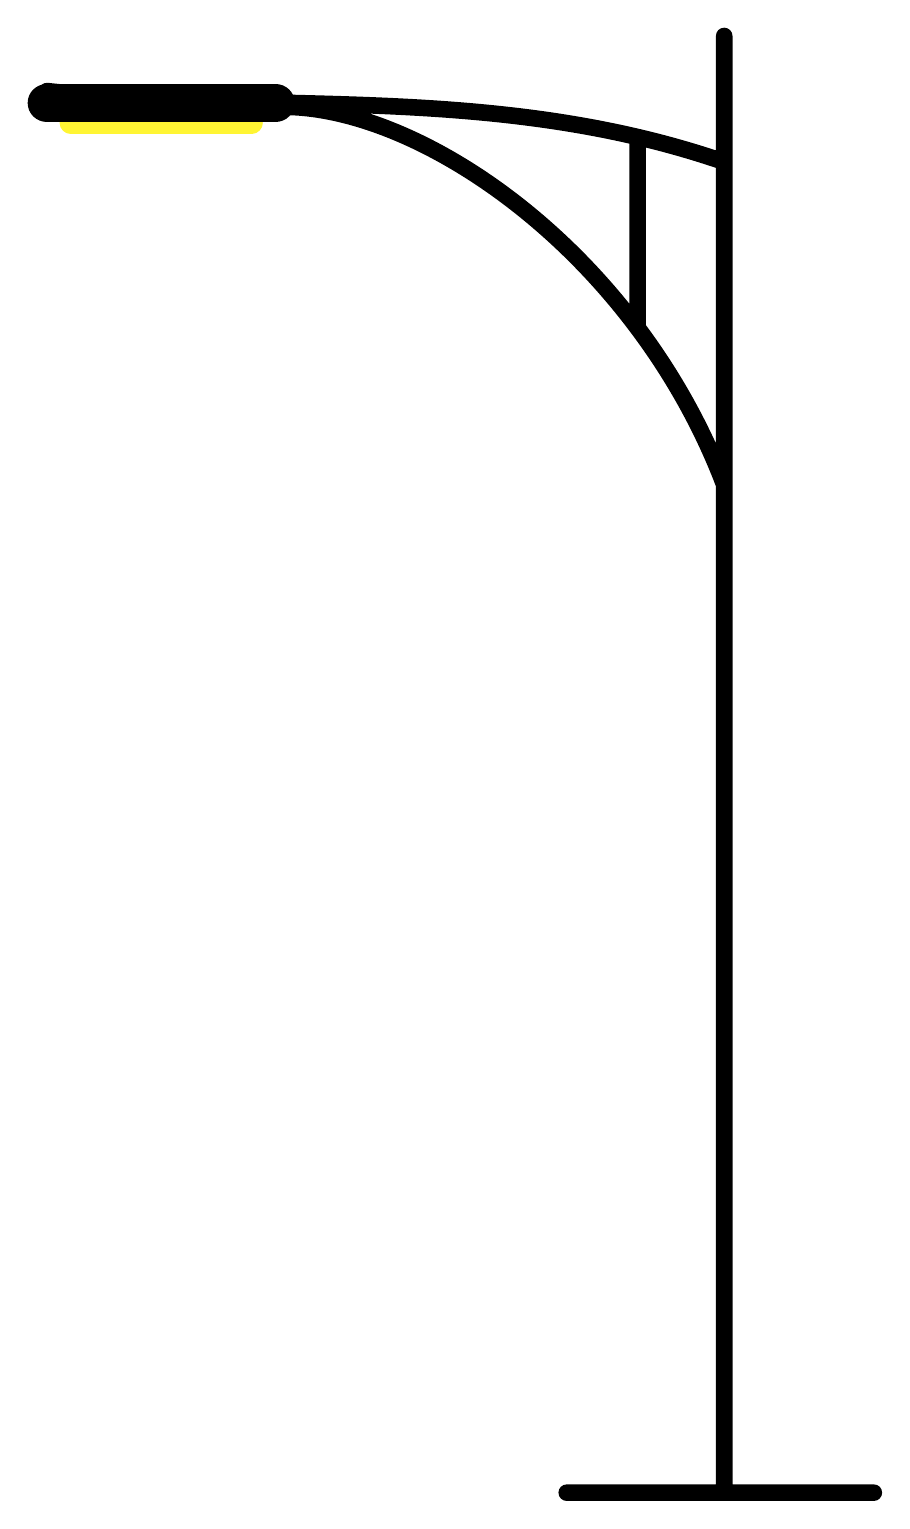
\begin{tikzpicture}[declare function={r=3;},font=\footnotesize, line join=round, line cap=round, >=stealth]
		\draw[yellow!80!white,line width=8] (0.3,17.4) -- (2.6,17.4);
		\draw[black,line width=6] (6.6,0) -- (10.5,0)(8.6,0) -- (8.6,18.5)(0,17.6) .. controls (1,17.6) and (1.7,17.6) .. (3,17.6) .. controls (4.8,17.6) and (7.5,15.7) .. (8.6,12.8)(8.6,16.9) .. controls (5.7,17.9) and (2.8,17.5) .. (0,17.8)(7.5,17.2) -- (7.5,14.8);
		\draw[black,line width=14] (0,17.65) -- (2.9,17.65);
	\end{tikzpicture}
\end{document}